%!TEX program = xelatex
\documentclass[aspectratio=169]{ctexbeamer}
% \usepackage{physics}  
                        %%% 宽高比说明 %%%%
%% ctexbeamer宏包支持各种宽高比,但本模板只适配了4:3(默认)和16:9的宽高比背景。
%% 添加选项aspectratio=169或aspectratio=43可以更改宽高比,默认是4:3
\usepackage[bluetheme]{ustcbeamer}
\usepackage{xcolor}
% !TeX root = ./main.tex

% 自适应16:9的宽高比设置
\makeatletter
\@ifclasswith{ctexbeamer}{aspectratio=169}{
		\def\backxscale{4/3}\def\backyscale{1}\def\ustcshift{30}
	}{
		\def\backxscale{1.068}\def\backyscale{1.068}\def\ustcshift{0}
	}
\makeatother

\newcommand{\maketitleframe}[1]{
	%取消footline,sidebar
	\setbeamertemplate{footline}[footlineoff]
	%%设置本命令以后的背景如下
	\usebackgroundtemplate{%
			\input{./theme/ustc_cover.tex}
	}%
	%封面页
	\begin{frame}%
		\maketitle%
		#1
	\end{frame}%
	%设置本命令以后的背景如下
	\usebackgroundtemplate{%
			\input{./theme/ustc_background.tex}
	}%
}%
%
\newcommand{\emptyline}{\newline\newline}
                        %%% ustcbeamer说明 %%%%
%% 宏包使用了TikZ代码形式的背景文件(在子文件夹theme中),默认选项"bluetheme",是科大校徽的蓝色;此外ustcbeamer还内置了红色和黑色主题"redtheme","blacktheme"。

                        %%% 自定义你的主题颜色 %%%
%% 一旦使用了下述命令就会覆盖ustcbeamer的内置颜色选项,你可以设置自己喜欢的RGB色值:
% \definecolor{themecolor}{RGB}{0,150,0} % 这是绿色主题
% \definecolor{themecolor}{RGB}{0,150,150} % 青色主题,也蛮好看的

%% 注意小写rgb和大写RGB表示的色值相差255倍,即RGB{255,255,255}=rgb{1,1,1};
% \definecolor{themecolor}{rgb}{0,0.5,0.3} % 深绿色主题

%% 建议自定义的主题颜色选择偏深色
%%%%%%%%%%%%%%%%%%%%%%%%%%%%%%%%%%%%%%%%%%%%%%%%%%%%%%%%%%%%%%%%%%%%%%


\title[Ko-Sched]{
  \textit{Ko-Sched}:一个离线的CUDA内核分割优化工具
}
\author[袁玉润]{报告人:袁玉润}
\institute[CS@USTC]{
中国科学技术大学\ 计算机科学与技术学院
}
\date{2023年6月7日}
\begin{document}
%\section<⟨mode specification⟩>[⟨short section name⟩]{⟨section name⟩}
%小于等于六个标题为恰当的标题

%--------------------
%标题页
%--------------------
\maketitleframe{\note{
  {\Large \textit{Ko-Sched}:一个离线的CUDA内核分割优化工具}
  \emptyline
  ko-Sched是一个使用搜索算法寻找CUDA程序的最佳配置的工具,致力于帮助开发人员在开发期优化其应用程序。
}}
%
%--------------------
%目录页
%--------------------
%beamer 101
% \begin{frame}%
% 	\frametitle{大纲}%
% 	\tableofcontents[hideallsubsections]%仅显示节
% 	%\tableofcontents%显示所节和子节
% \end{frame}%
%--------------------
%节目录页
%--------------------
\AtBeginSection[]{
\setbeamertemplate{footline}[footlineoff]%取消页脚
  \begin{frame}%
    \frametitle{目录}
	%\tableofcontents[currentsection,subsectionstyle=show/hide/hide]%高亮当前节,不显示子节
    \tableofcontents[currentsection,subsectionstyle=show/show/hide]%show,shaded,hide
  \end{frame}
\setbeamertemplate{footline}[footlineon]%添加页脚
}
%--------------------
%子节目录页
%--------------------
\AtBeginSubsection[]{
\setbeamertemplate{footline}[footlineoff]%取消页脚
  \begin{frame}%
    \frametitle{目录}
	%\tableofcontents[currentsection,subsectionstyle=show/hide/hide]%高亮当前节,不显示子节
    \tableofcontents[currentsection,subsectionstyle=show/shaded/hide]%show,shaded,hide
  \end{frame}
\setbeamertemplate{footline}[footlineon]%添加页脚
}

\section{研究背景}
\begin{frame}
  \frametitle{CUDA编程}
  \begin{columns}
    \begin{column}{0.4\textwidth}
      \begin{itemize}
        \item NVIDIA 并行计算架构
        \item CUDA程序包括主机(host)代码和设备(device)代码 \\
        \begin{itemize}
          \item 主机代码:运行在CPU上,负责管理设备内存,调用设备代码
          \item 设备代码(内核/kernel):运行在GPU上,负责执行计算任务
        \end{itemize}
      \end{itemize}
    \end{column}
    \begin{column}{0.60\textwidth}
      \begin{figure}
        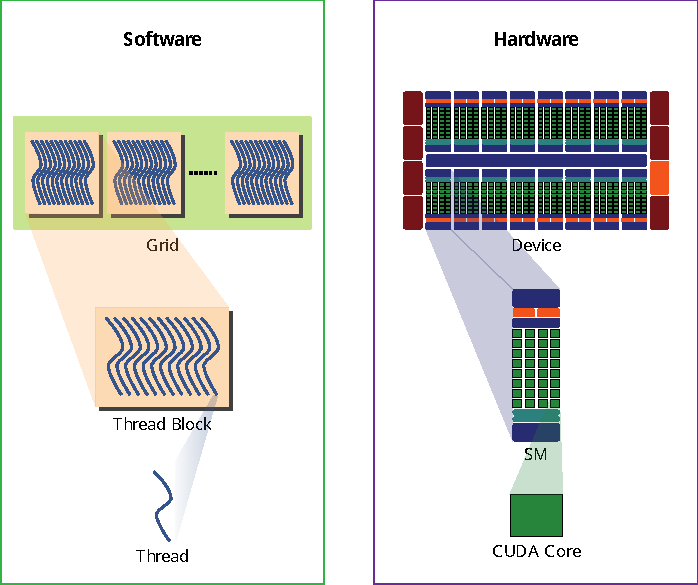
\includegraphics[width=\textwidth]{figures/programming_model_executing_model.pdf}
        % \caption{CUDA编程模型与执行模型的对应关系}
      \end{figure}
    \end{column}
  \end{columns}
  \note{
    首先介绍一些CUDA编程的相关知识。
\emptyline
    一个CUDA程序包括在CPU上执行的主机代码和在GPU上执行的设备代码,即内核。
\emptyline
    在内核执行时,许多线程并行执行相同的设备代码。几十至上百个线程组成一个线程块。%,每个内核由多个线程块组成。
\emptyline
    在内核启动后,每个线程块会被分配到GPU上的一个流处理器(即SM)上执行。%SM内的CUDA core会执行线程块中的线程。
  }
\end{frame}


\begin{frame}
  \frametitle{线程块的调度策略}
  \begin{columns}
    \begin{column}{0.4\textwidth}
      \begin{itemize}
        \item 每个线程块(thread block)被分配到1个流处理器(SM)上执行
        \item 多个kernel启动后,GPU将首个kernel的线程块逐个分配给SM
        \item 若在分配完毕后设备仍有剩余硬件资源则开始分配下一个kernel
      \end{itemize}
    \end{column}
    \begin{column}{0.60\textwidth}
      \scriptsize{\begin{figure}
        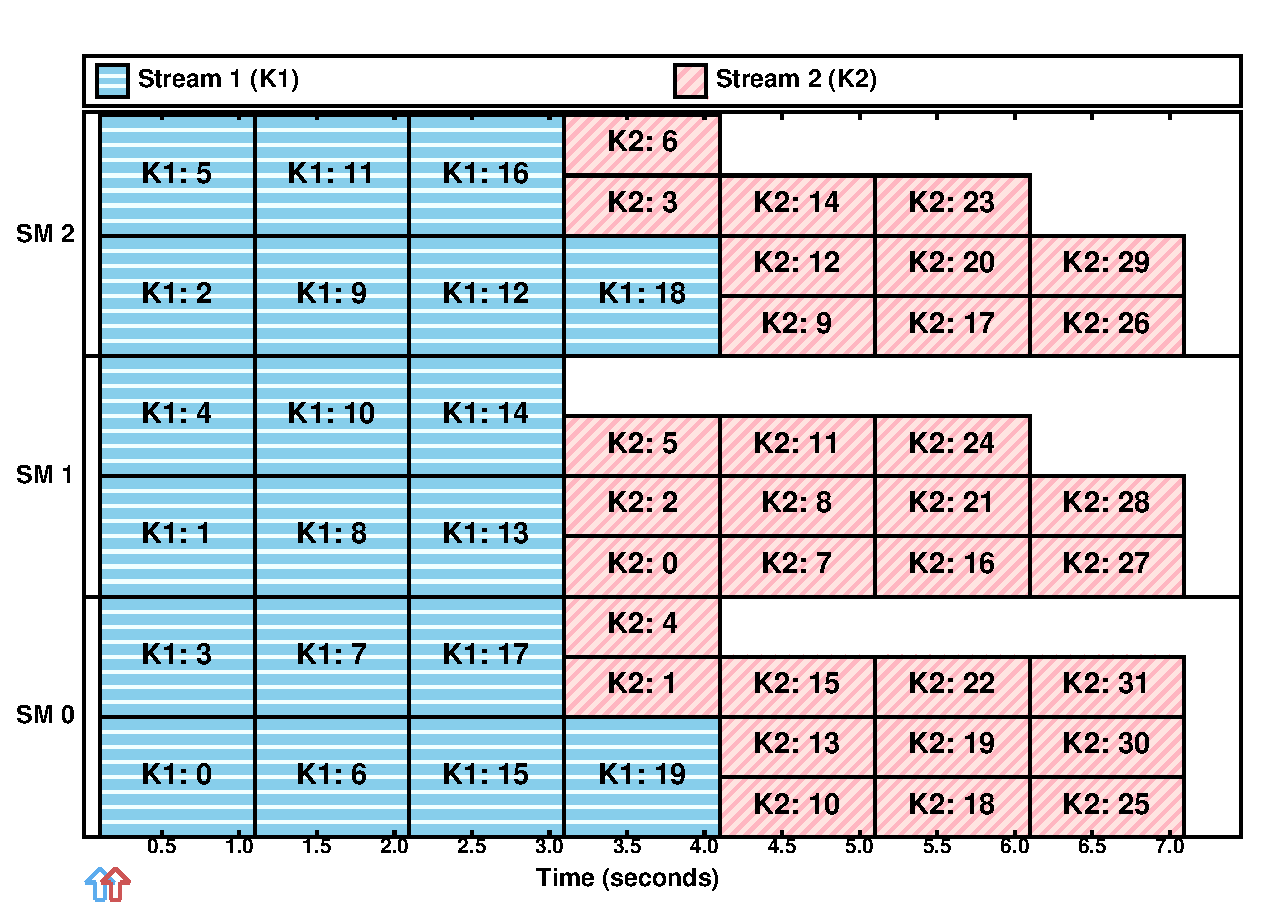
\includegraphics[width=\textwidth]{figures/kernel_nonparallel.pdf}
        \caption{内核$K1$,$K2$的线程块分配到流处理器的情况}
      \end{figure}}
    \end{column}
  \end{columns}
  \note{
    当有多个内核依此启动时,GPU会首先将第一个内核的线程块逐个分配给SM。若分配完后仍有剩余的硬件资源,则开始分配第二个内核的线程块。
\emptyline
    {\large 图.}右图展示了2个内核依此启动后线程块分配到SM上的情况,图中蓝色矩形代表kernel1的线程块,粉色矩形代表kernel2的线程块,横轴为时间,纵轴为不同的SM。
\emptyline
    可以看到,kernel1的线程块会首先被分配,全部分配完成后kernel2的线程块才会开始分配。
  }
\end{frame}

\begin{frame}
  \frametitle{内核分割}
  \begin{itemize}
    \item \textbf{问题}:若2个kernel具有不同资源瓶颈,其低并行度导致GPU资源利用率低。\\
    e.g. 计算密集型kernel与内存密集型kernel
    \begin{figure}
      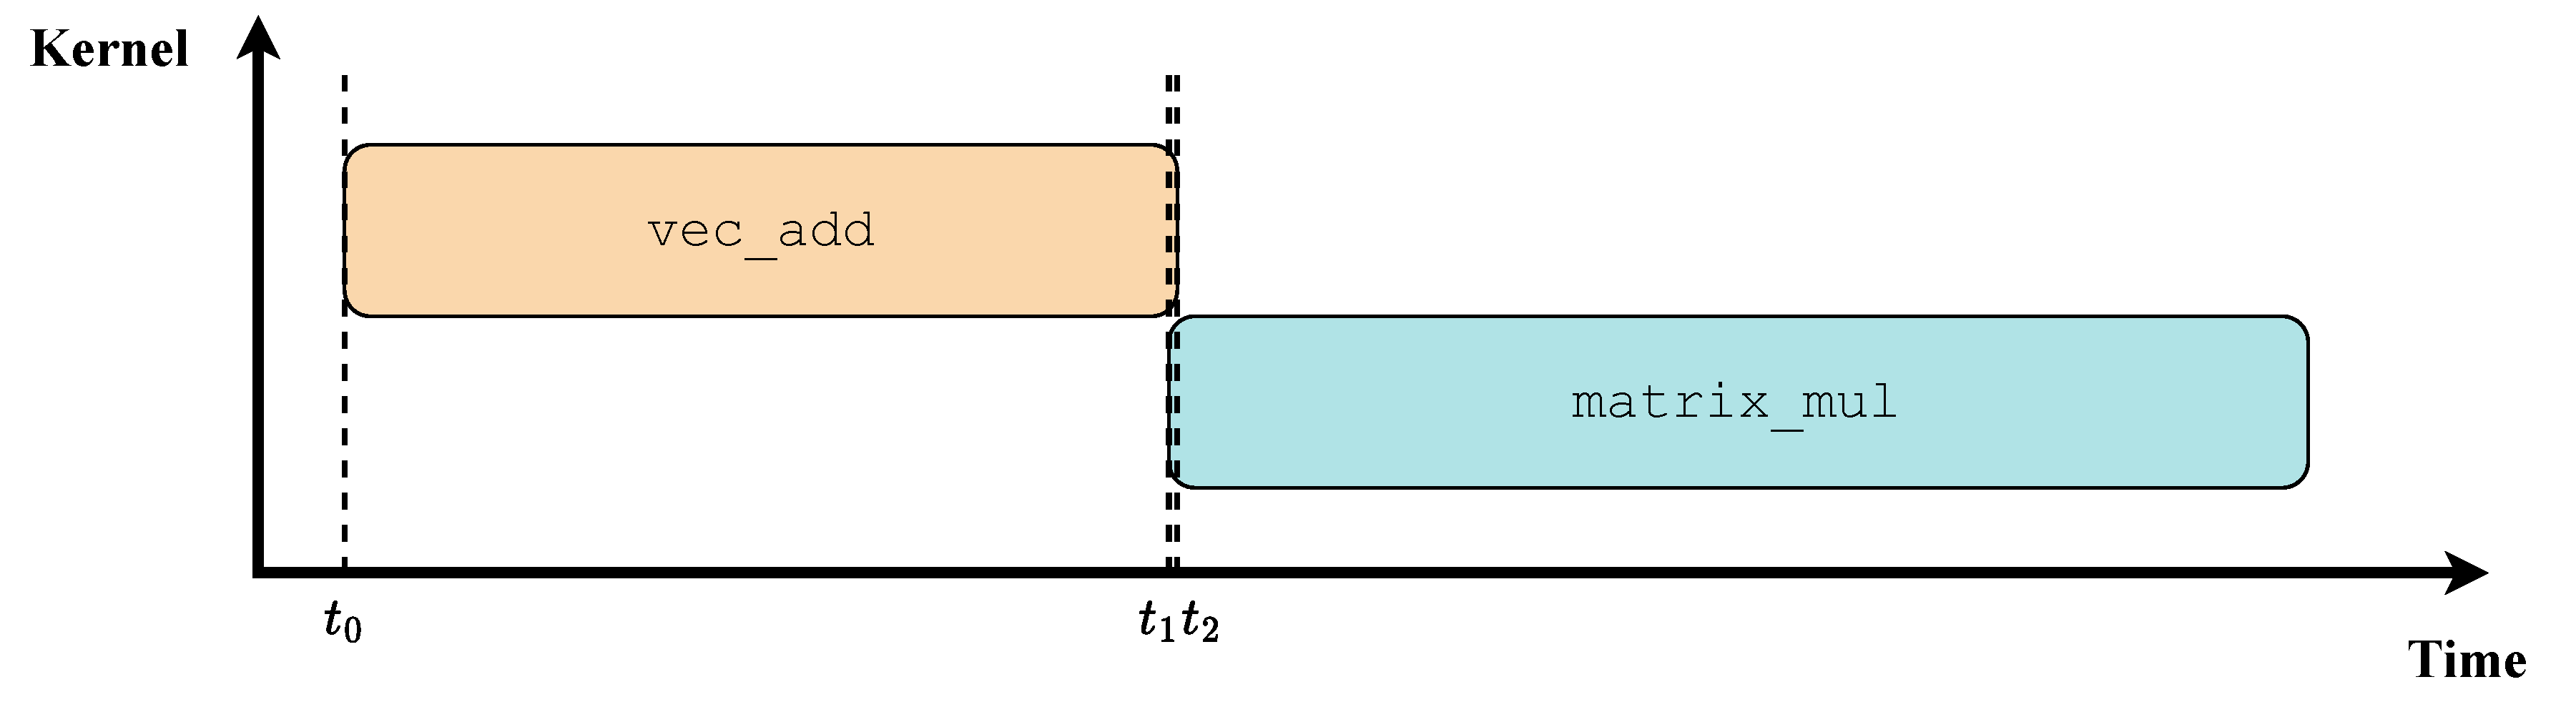
\includegraphics[width=0.6\textwidth]{figures/serial_execution.drawio.pdf}
    \end{figure}
    \item \textbf{解决}:将kernel分割成多个子内核,使得不同kernel的子内核间并行,从而实现不同kernel的并行
    \begin{figure}
      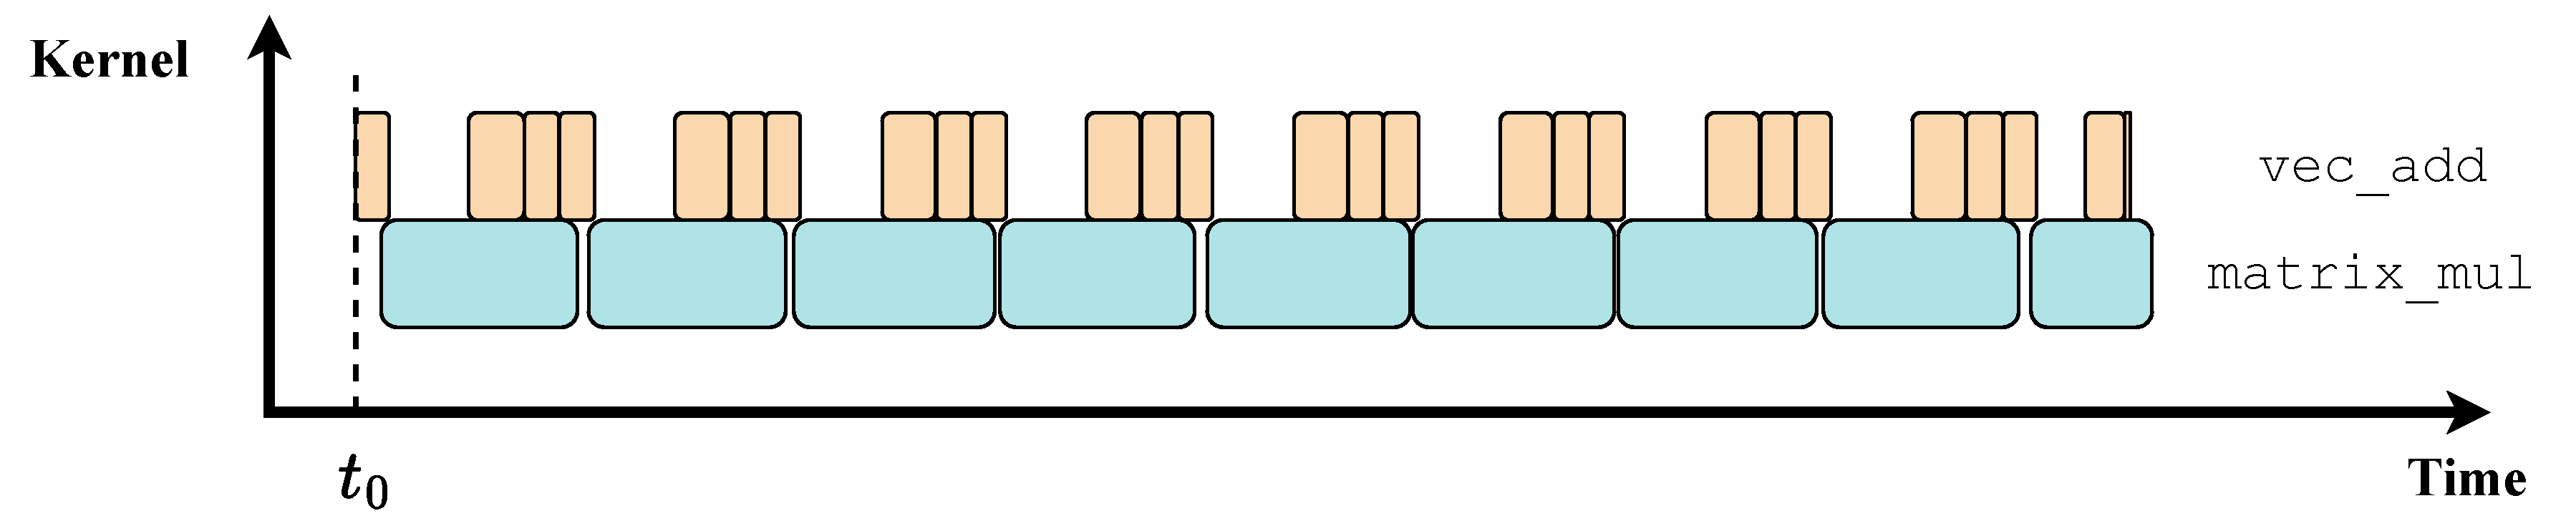
\includegraphics[width=0.6\textwidth]{figures/opt_cosched.drawio.pdf}
    \end{figure}
  \end{itemize}
  \note{
    这种调度策略带来的问题是,当多个内核启动时,不同内核间的并行度很低。而有时不同内核并行可以带来显著的性能提升。例如,一个内存密集型内核与一个计算密集型内核并行可提高GPU硬件的利用率,从而降低总执行时间。
    \emptyline
    为解决这个问题,一种主流方法是将内核切分为多个较小的子内核,即内核分割技术。这样,当某个子内核分配完毕后,GPU仍有剩余资源分配给另一个子内核,实现了不同内核的并行。
  }
\end{frame}

\begin{frame}
  \frametitle{问题}
  \textbf{新问题}:子内核大小的选择
  \begin{itemize}
    \item 子内核过大:单个子内核占用GPU资源过多,导致其他子内核无法并行执行
    \item 子内核过小:启动子内核次数较多,启动开销较大
  \end{itemize}
  \footnotesize{\begin{figure}
    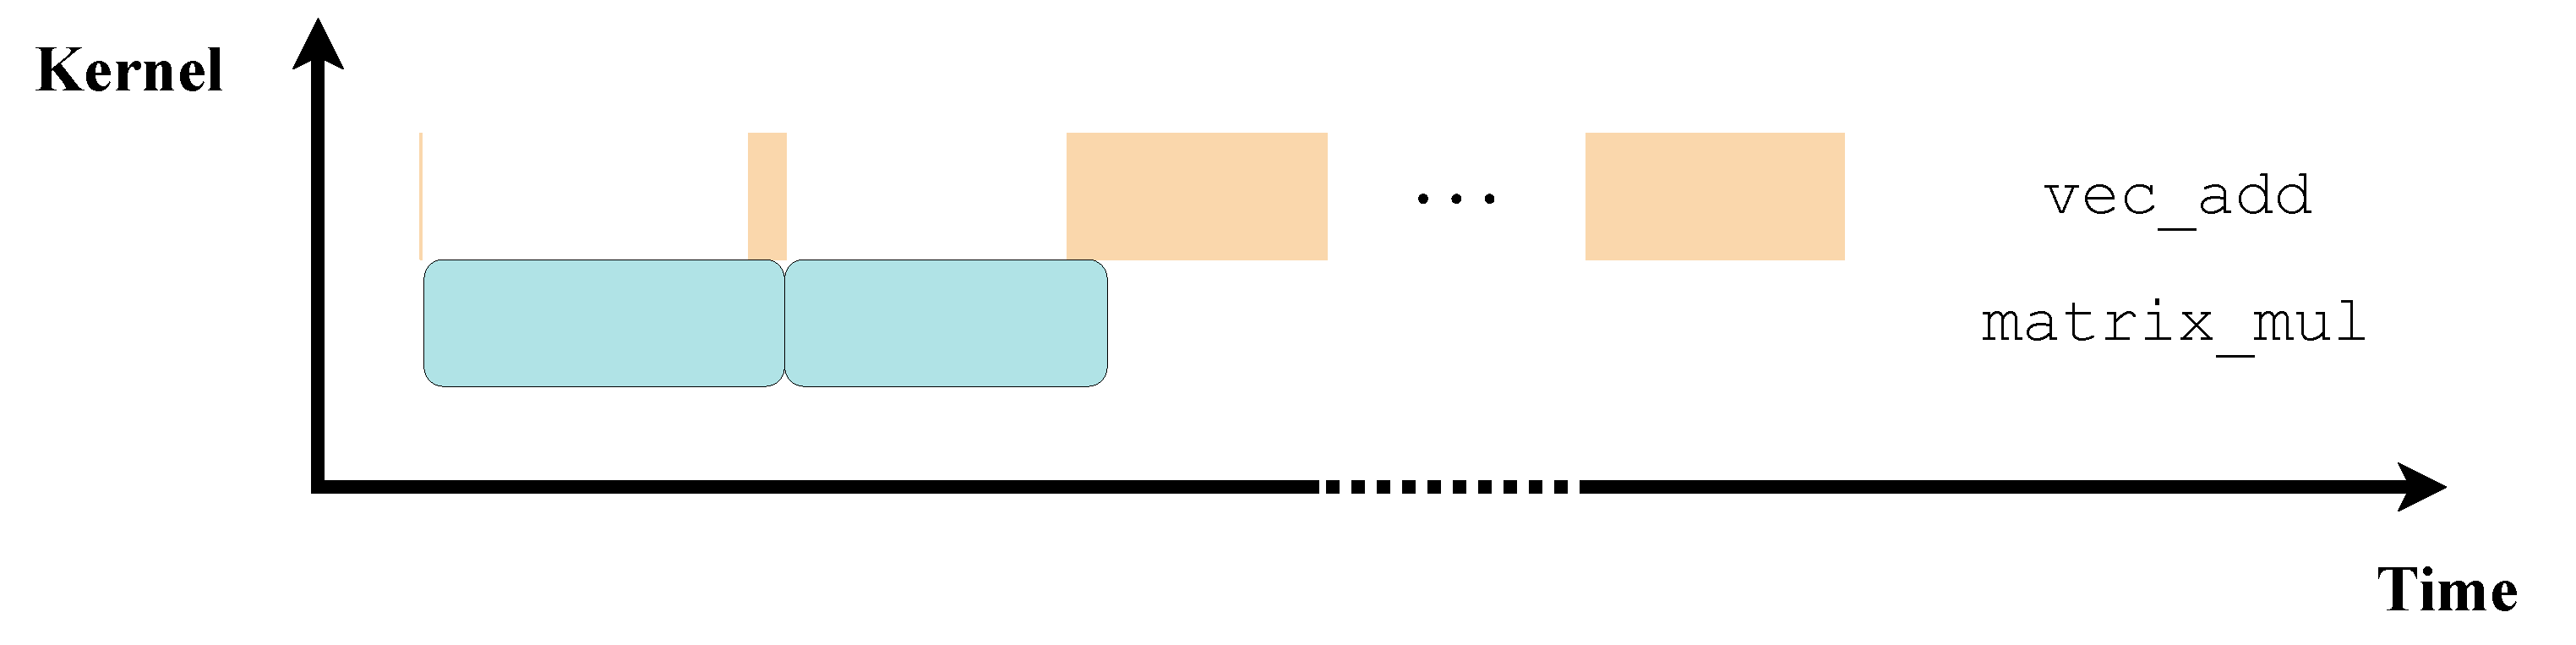
\includegraphics[width=0.7\textwidth]{figures/bad_cosched.drawio.pdf}
    \caption{错误的分割方式使得 kernel 并未实现并行,反而引入了多次内核启动的开销,使得性能低于未分割内核的情况。}
  \end{figure}}
  \note{
    然而,使用内核分割会带来的新问题,即如何确定子内核的大小。

    \begin{itemize}
      \item 较大的子内核可能会占用过多的GPU资源,导致其他子内核无法并行执行
      \item 而较小的子内核会使子内核数目变多,增加内核启动开销
    \end{itemize}
  }
\end{frame}

\begin{frame}
  \frametitle{动机}
  \textbf{发现}:分割参数变化时,程序性能的变化具有连续性
  \begin{columns}
    \begin{column}{0.5\textwidth}
      \begin{flushright}
        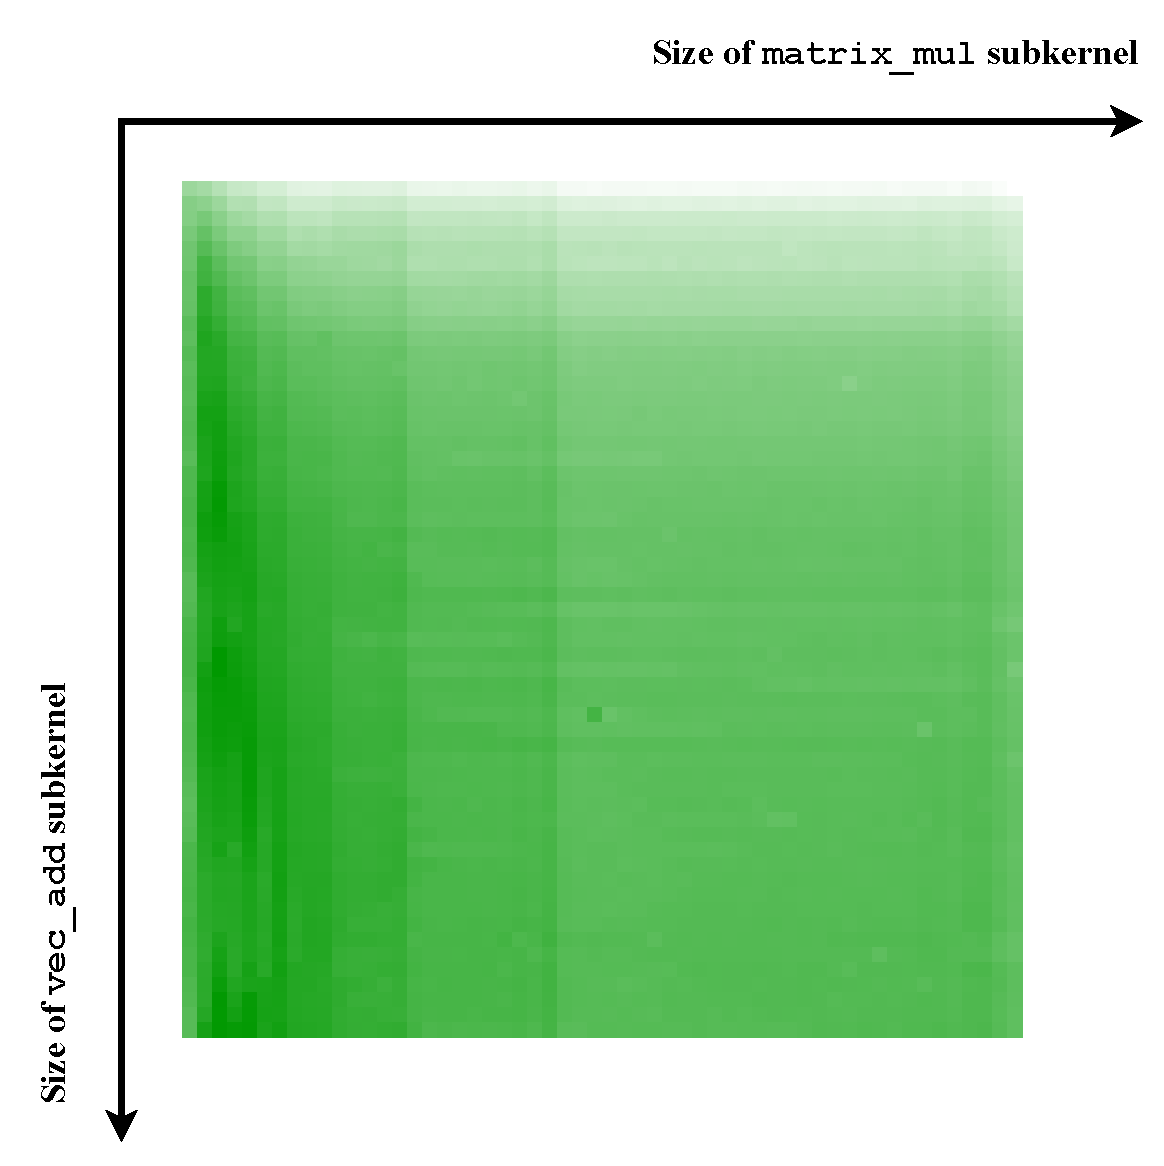
\includegraphics[width=0.67\textwidth]{figures/consistency.drawio.pdf}
      \end{flushright}
    \end{column}
    \begin{column}{0.5\textwidth}
      \footnotesize{如图,纵轴表示内核\texttt{vec\_add}的子内核大小,横轴表示内核\texttt{matrix\_mul}的子内核大小。\\
      每个坐标对应的方格颜色表示在此分割参数的组合下的程序性能,颜色越深表示性能越高。}
    \end{column}
  \end{columns}

  \textbf{启发}:可以类比数值计算中求解函数极值的算法(如梯度下降)来寻找性能较高的配置,而无需遍历地测试每一种可能的分割方式

  \note{
    为解决这个问题,我们探究了程序性能与子内核大小的关系。
    \emptyline
    如图,纵轴表示矢量加法程序(\texttt{vec\_add})的子内核大小,横轴表示矩阵乘法(\texttt{matrix\_mul})的子内核大小。每个绿色方格颜色表示在此分割参数的组合下的程序性能,颜色越深表示性能越高。
    \emptyline
    图中信息表明,当分割参数变化时,程序性能的变化具有连续性。
    %即,当分割参数发生微小变化时,程序性能也会相应发生微小变动,而不会出现剧烈的波动。
    这种连续性允许我们类比求解函数极值的算法(如梯度下降)来寻找性能较高的配置,而无需遍历地测试每一种可能的分割方式。
  }
\end{frame}

\section{算法设计}
\begin{frame}
  \frametitle{算法流程}
  \begin{columns}
    \begin{column}{0.5\textwidth}
      \begin{block}{}
        \indent
        \begin{enumerate}
          \item 随机选取初始子内核大小
          \item 测量若干个与此配置相近配置的性能
          \item 选取性能最高者为新的基准配置
          \item 重复上述操作直到当前基准配置优于所有相近配置
        \end{enumerate}
      \end{block}
      Ko-Sched将多次选取初始配置重复上述流程,选取最佳结果
    \end{column}
    \begin{column}{0.5\textwidth}
      \begin{figure}
        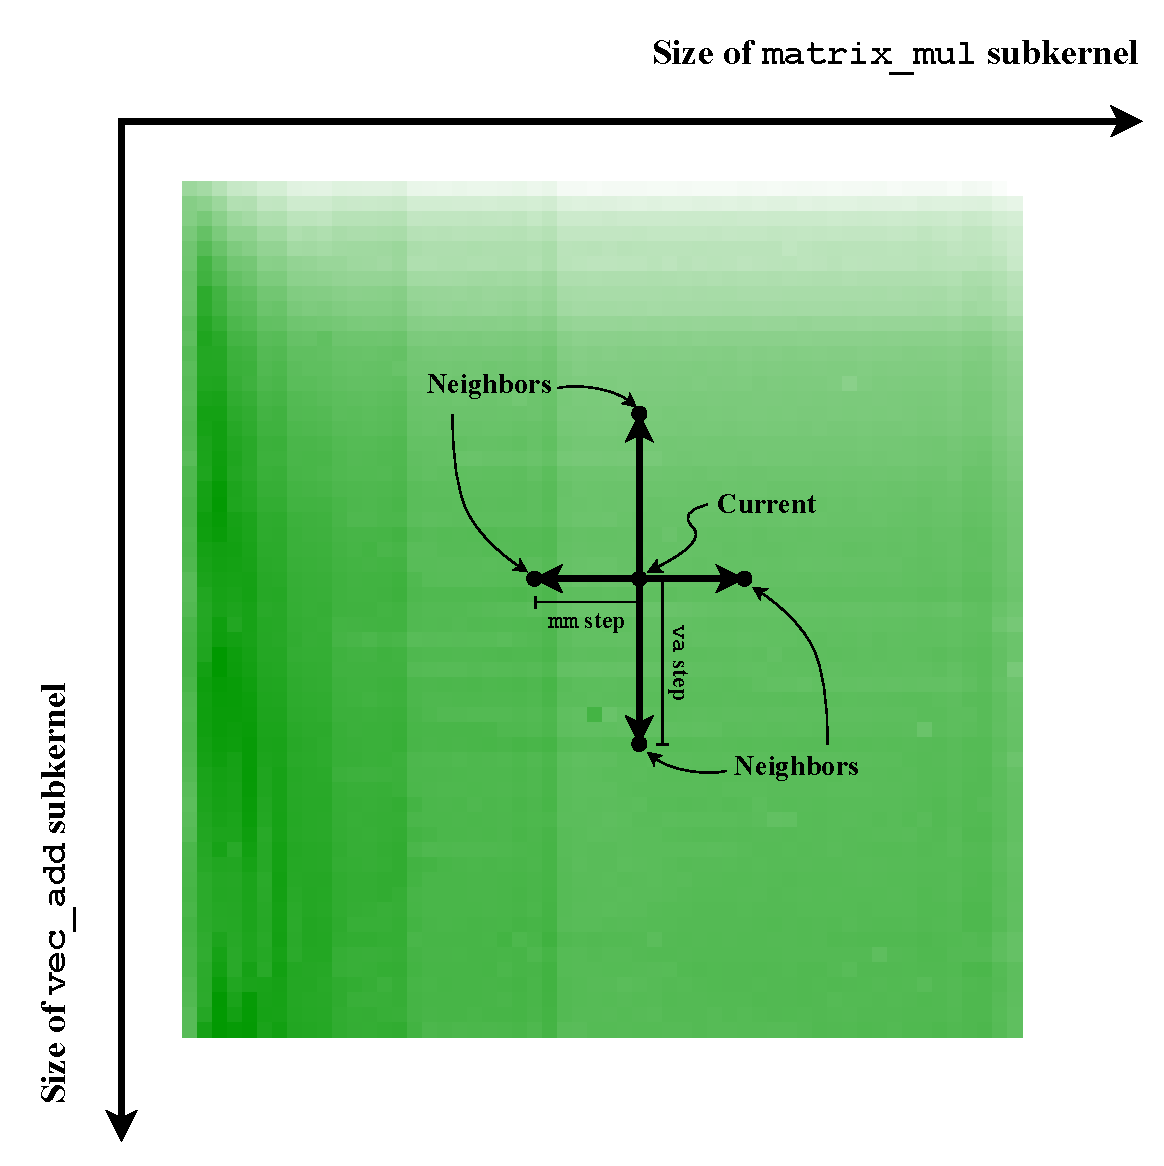
\includegraphics[width=0.9\textwidth]{figures/searching_concept.drawio.pdf}
      \end{figure}
    \end{column}
  \end{columns}
  \note{
    因此,我们设计了如下算法:
    \emptyline
    \textit{verbatim}
  }
\end{frame}

\begin{frame}
  \frametitle{可变搜索步长}
  \begin{columns}
    \begin{column}{0.5\textwidth}
    \textbf{问题}
      \begin{itemize}
        \item 过小的步长会使算法收敛于局部最优解
        \item 过大的步长可能使算法在调整参数时忽略最优解
      \end{itemize}
    \textbf{解决}
      \begin{itemize}
        \item 先使用较大步长快速定位至性能高的参数区域
        \item 之后以小步长在此区域寻找精准优解
      \end{itemize}
    \end{column}
    \begin{column}{0.5\textwidth}
      \begin{figure}
        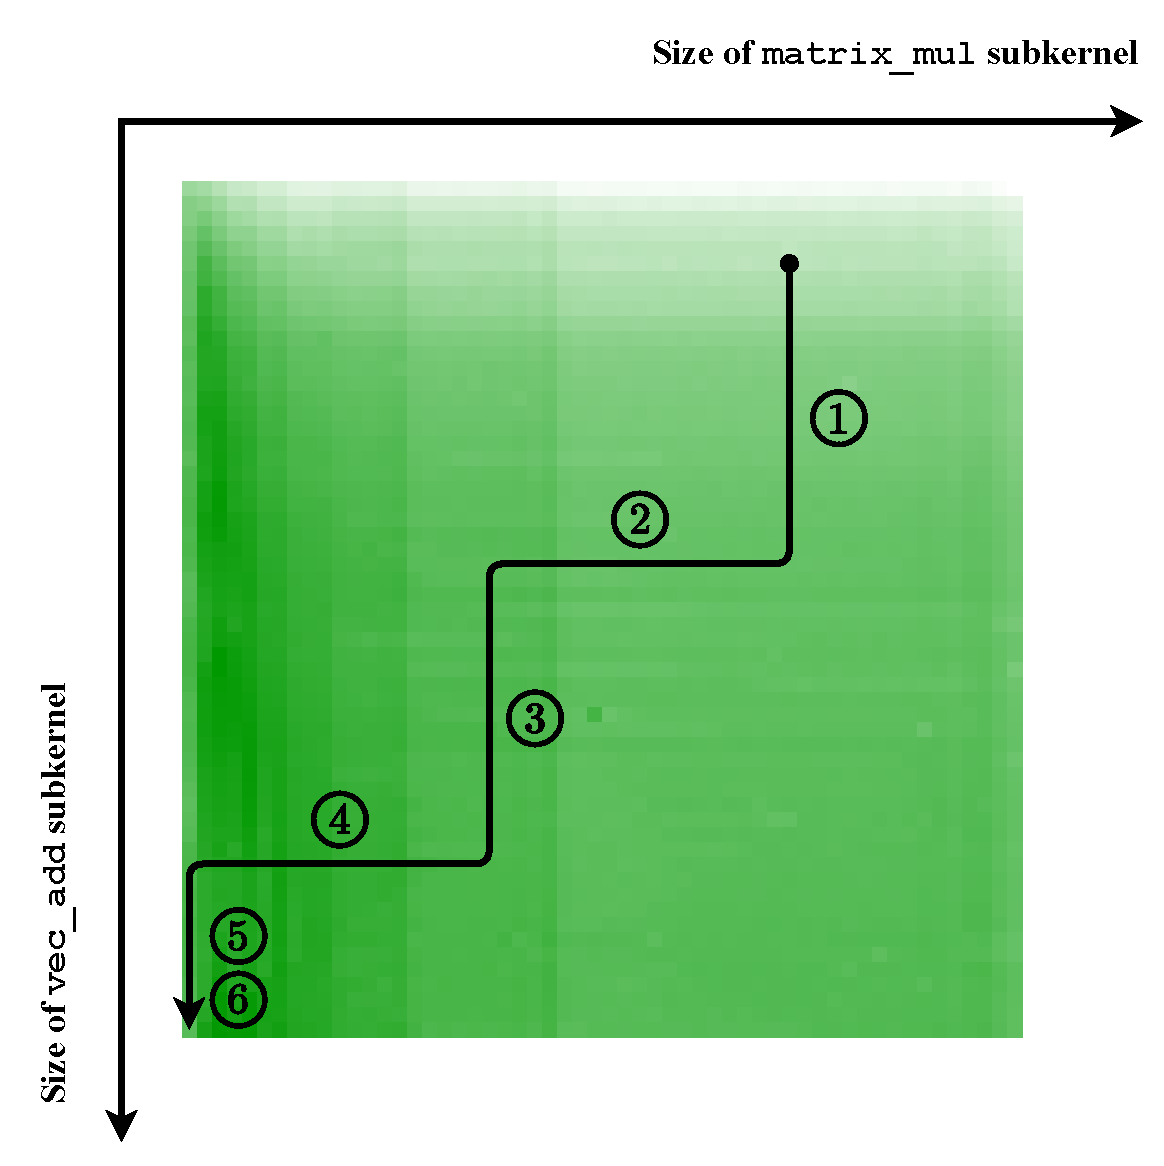
\includegraphics[width=0.9\textwidth]{figures/searching_trace_va_mm.drawio.pdf}
      \end{figure}
    \end{column}
  \end{columns}
  \note{
    在搜索算法,中每次调整的步长的选择十分关键。
    \emptyline
    \textit{verbatim}
    \emptyline
    右图展示了实际执行的一次搜索结果,ko-Sched快速定位到了较优的配置。
  }
\end{frame}

\begin{frame}
  \frametitle{分析给定分割配置下的性能}
      通过测量部分子内核的执行时间估算此配置下的完整运行时间。
      % \emptyline
      % 如图,启动kernel 1的1个子内核与kernel 2的3个子内核,视这部分执行时间的3倍为估算的完整运行时间。
      % $N^1_{\text{subkernel}}$倍为完整运行时间的估算。其中$N^1_{\text{subkernel}}$为kernel 1的子内核数目。
      \begin{center}
        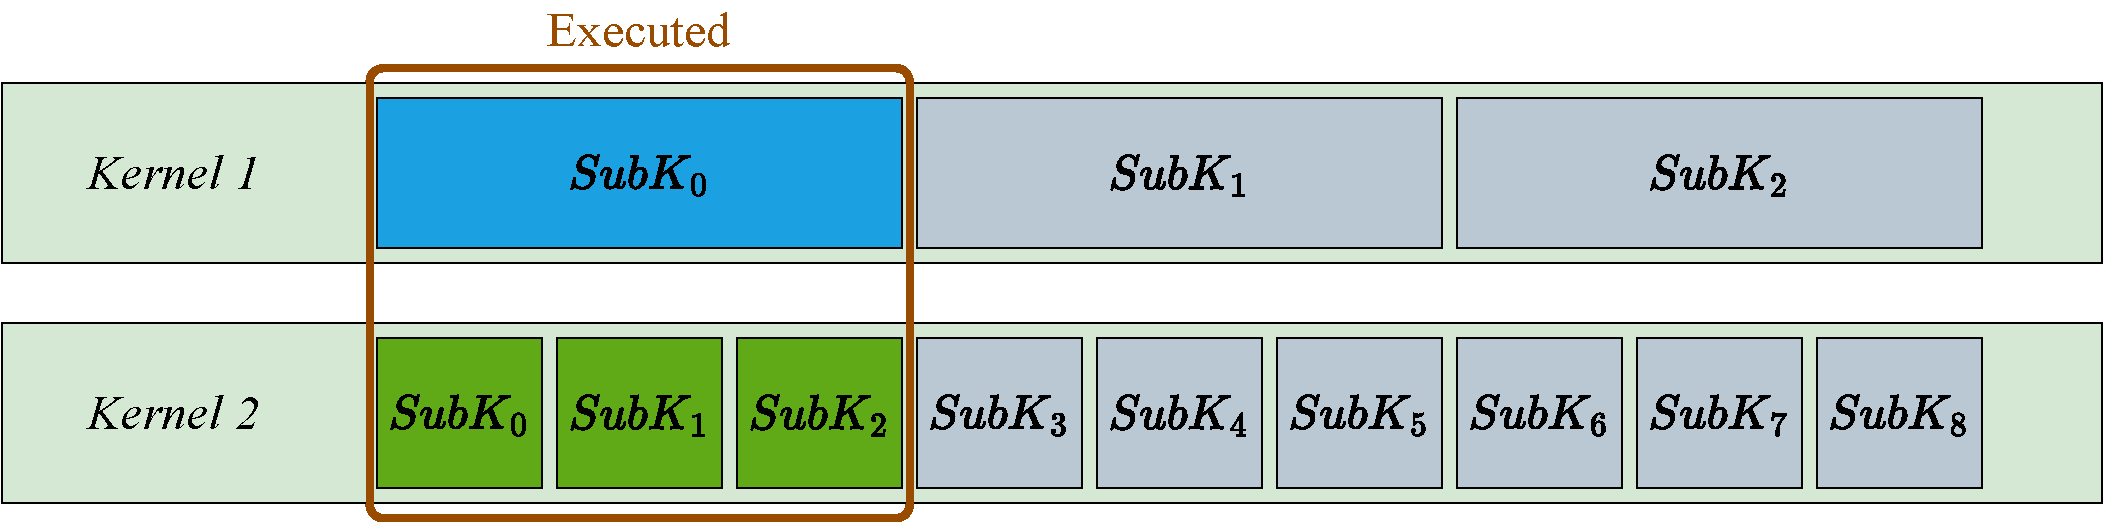
\includegraphics[width=0.9\textwidth]{figures/sampling.drawio.pdf}
      \end{center}
      \note{
        搜索算法中需要测量某一配置的性能。为了能以较低开销获得准确的性能,ko-Sched测量2个内核的部分子内核的执行时间来估算完整运行时间。
        % \emptyline
        % 例如,对具有3个子内核的内核1和9个内核的内核2,可以启动1个内核1的子内核和3个内核2的子内核,并以执行时间的3倍作为完整运行时间的估计。
      }
\end{frame}

\section{实验测试}
\begin{frame}
  \frametitle{实验环境}
  \begin{columns}
    \begin{column}{0.6\textwidth}
    \large{测试程序}
      \begin{itemize}
        \item {\color{blue}{\texttt{matrix\_mul}} (\texttt{mm})}\ 矩阵乘法内核
        \item {\color{blue}{\texttt{vec\_add}} (\texttt{va})}\ 矢量加法内核
        \item {\color{blue}{\texttt{matrix\_transpose}} (\texttt{mt})}\ 矩阵转置内核
        \item {\color{blue}{\texttt{sqrt\_pow}} (\texttt{sp})}\ 一个运算密集型内核,每个线程进行大量的平方根和指数运算。
      \end{itemize}
    \end{column}
    \begin{column}{0.45\textwidth}
      \large{实验涉及GPU硬件}
      \begin{itemize}
        \item NVIDIA GeForce MX250
        \item NVIDIA GeForce RTX 2080Ti
        \item NVIDIA GeForce RTX 3080
        \item NVIDIA GeForce RTX 3090
      \end{itemize}
      \ \\
    \end{column}
  \end{columns}
  \note{
    为测试ko-Sched效果,我们实现了4个测试程序并在4个型号的GPU上实验。
  }
\end{frame}

\begin{frame}
  \frametitle{相对于未分割版本的性能}

  \scriptsize{\begin{center}
    \begin{figure}
      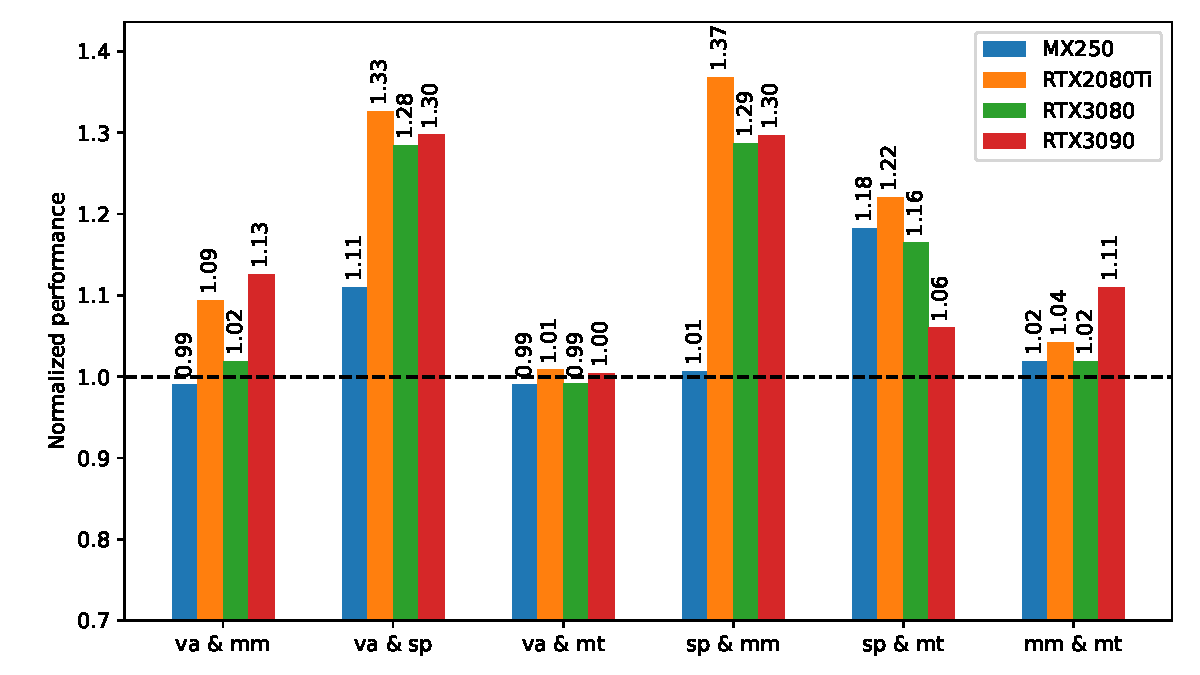
\includegraphics[width=0.7\textwidth]{figures/perf-eval-diff-dev.pdf}
      \caption{在不同GPU上ko-Sched相对于未分割版本的性能。平均提升达$12.5\%$}
    \end{figure}
  \end{center}}
  \note{
    首先我们对比了使用ko-Sched相较于未分割内核的原始版本的性能。可见ko-Sched在绝大部分情形下带来了性能提升,平均提升到12.5\%,在部分场景下甚至能达到30\%。
  }
\end{frame}

\begin{frame}
  \frametitle{相对于最佳分割参数下的性能}

  \scriptsize{\begin{center}
    \begin{figure}
      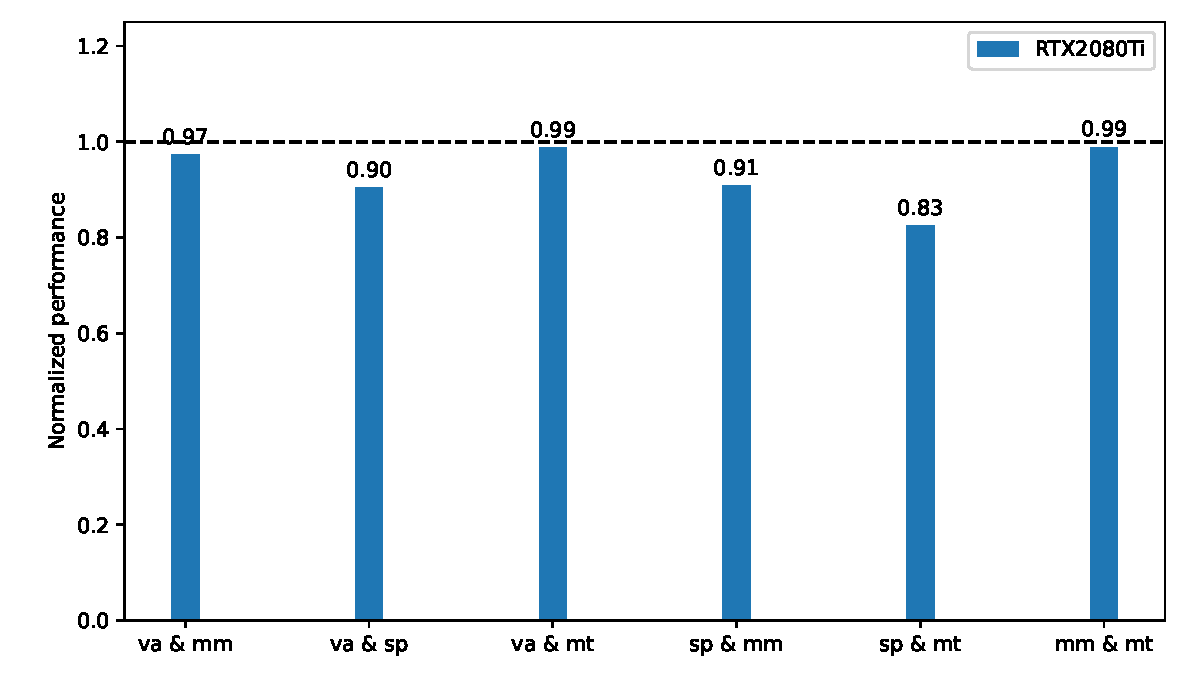
\includegraphics[width=0.7\textwidth]{figures/perf-eval-compared-to-opt.pdf}
      \caption{ko-Sched相对于遍历搜索得到的最佳分割参数的性能。平均达到$ 93.14\%$}
    \end{figure}
  \end{center}}

  \note{
    此外,我们遍历了大量的分割参数下的程序性能,找到了其中性能最佳的参数组合,并将ko-Sched的性能与之比较。可见,ko-Sched 算法所得结果的性能与最优结果的性能相差不大,平均达到了最佳性能的93.14\%。
  }
\end{frame}


\begin{frame}
  \frametitle{相对于搜索时准确测量执行时间的算法的性能}

  \scriptsize{\begin{center}
    \begin{figure}
      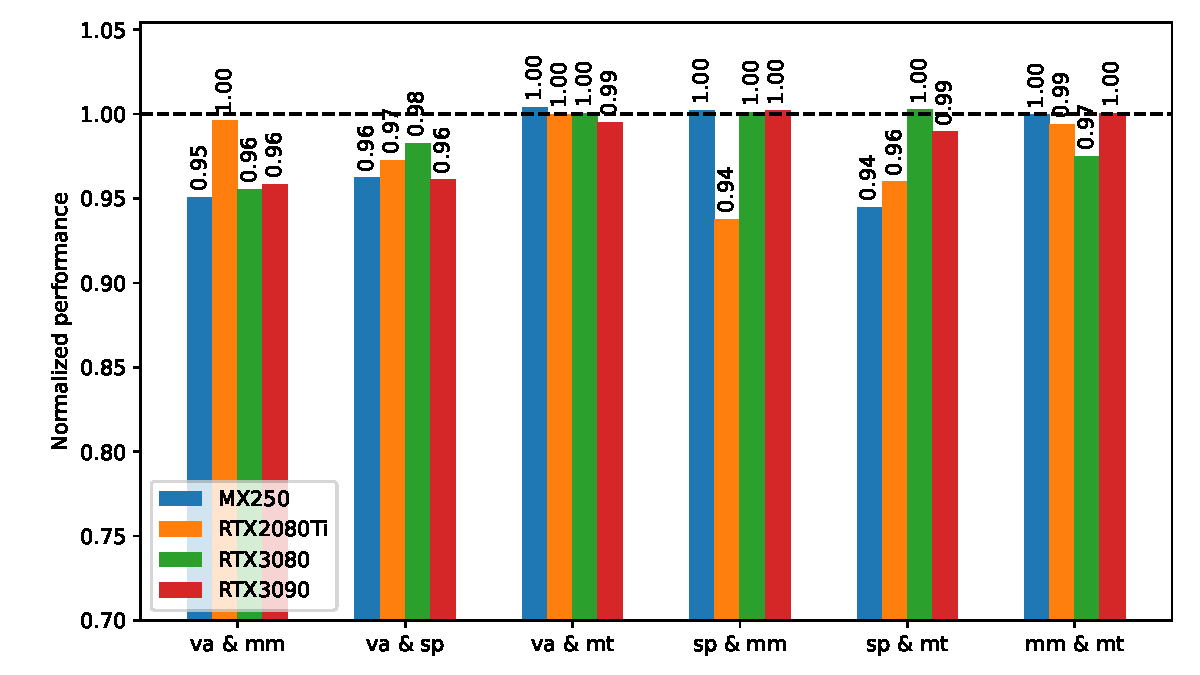
\includegraphics[width=0.7\textwidth]{figures/perf-eval-compared-to-nonsampling.pdf}
      \caption{ko-Sched相对于变种ko-Sched'的性能;ko-Sched'在搜索时准确测量执行时间。平均达到$98.12\%$}
    \end{figure}
  \end{center}}
  \note{
    最后,我们想要说明使用估算的方法测量某分割参数下的执行时间不会对最后结果有明显影响。我们实现了 ko-Sched 的变种,ko-Sched’,它在搜索时执行所有子内核并记录准确的执行时间,因而得到的搜索结果会更加准确。可以看到,ko-Sched的结果与ko-Sched’的结果相差不大,在所有测试程序中平均达到了ko-Sched'的98.12\%。
  }
\end{frame}

\begin{frame}
  \centerline{\Large 谢谢!}
\end{frame}

\end{document}
